 % TEX-option: shell-escape
\documentclass{article} % For LaTeX2e
\usepackage{nips15submit_e,times}
\usepackage{hyperref}
\usepackage{url}
\usepackage{graphicx}
\usepackage{amssymb}
\usepackage{amsmath}
\usepackage{subcaption}
\usepackage{listings}
\usepackage{algorithm2e}
\usepackage[numbib]{tocbibind}



\usepackage{courier}
\lstset{basicstyle=\footnotesize\ttfamily,breaklines=true}
\lstset{framextopmargin=50pt,frame=bottomline}
%\documentstyle[nips14submit_09,times,art10]{article} % For LaTeX 2.09


\title{Conformal Parameterization of a surface}


\author{
Chi Po Choi \\
Department of Statistics\\
University of California, Davis\\
\texttt{cpchoi@ucdavis.edu} \\
}

% The \author macro works with any number of authors. There are two commands
% used to separate the names and addresses of multiple authors: \And and \AND.
%
% Using \And between authors leaves it to \LaTeX{} to determine where to break
% the lines. Using \AND forces a linebreak at that point. So, if \LaTeX{}
% puts 3 of 4 authors names on the first line, and the last on the second
% line, try using \AND instead of \And before the third author name.

\newcommand{\fix}{\marginpar{FIX}}
\newcommand{\new}{\marginpar{NEW}}

\nipsfinalcopy % Uncomment for camera-ready version

\begin{document}

\maketitle

\begin{abstract}
We computationally construct a conformal parameterization of a surface. We only consider the surface which is topologically equivalent to 2-dimensional disk. In other words, the surface is orientable, simply-connected and has only one boundary curve. We aim to find a conformal parameterization the surface onto a unit disk, with the boundary curve lying on the unit circle. This parameterization can be obtained by solving a Laplace equation with suitable boundary condition. The surface is discretized as a triangle mesh. Solving this Laplace equation is formulated as an optimization problem which has a quadratic objective with quadratic and linear constraints. We solve the optimization problem using augmented Lagrangian method.
\end{abstract}

\section{Introduction}

One picture worths more than thousands of words. Figure 1 illustrates the goal of this final project. See Figure 1. Figure 1(a) is a surface mesh of a hat. This surface is topologically equivalent to a disk. We want to find a  parameterization of the surface on a unit disk, with the boundary curve of the surface lying on the unit circle. Figure 1(b) is a example of parameterization of this surface mesh. We can regard parameterization as a process of flattening the triangle mesh from 3D space to 2D plane. However, not any parameterization is useful. We want a special kind of surface parameterization: conformal parameterization, which preserves the angles of the triangle. Figure 1(c) is an example of conformal parameterization of this surface mesh. The angles of the triangles on the Figure 1(c) match those on the surface mesh, while those on Figure 1(b) does not.

\begin{figure}[h!]
        \centering
        \begin{subfigure}[b]{0.4\textwidth}
                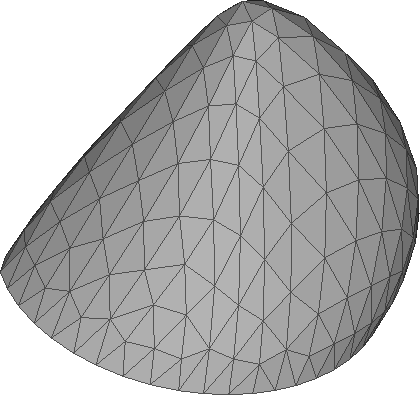
\includegraphics[width=\textwidth]{f1a.png}
                \caption{Surface mesh of a hat}
                \label{fig:pargraph}
        \end{subfigure} \\
        \begin{subfigure}[b]{0.4\textwidth}
                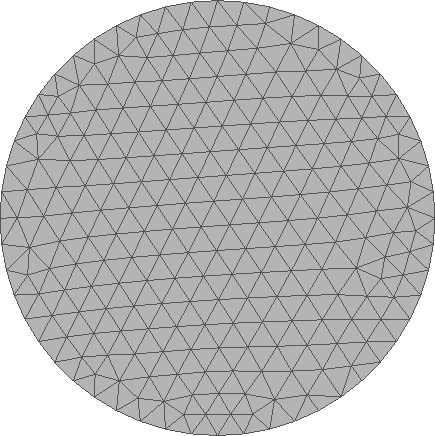
\includegraphics[width=\textwidth]{f1c.png}
                \caption{*NOT* conformal parameterization}
                \label{fig:pargraph}
        \end{subfigure}
        \begin{subfigure}[b]{0.4\textwidth}
                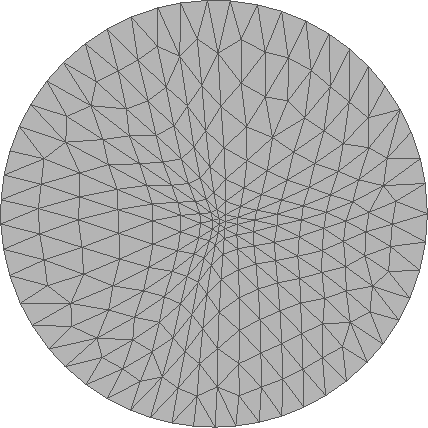
\includegraphics[width=\textwidth]{f1b.png}
                \caption{Conformal parameterization}
                \label{fig:parconf}
        \end{subfigure}
        ~ %add desired spacing between images, e. g. ~, \quad, \qquad, \hfill etc.
          %(or a blank line to force the subfigure onto a new line)
        \caption{Conformal Parameterization}\label{fig:footpar}
\end{figure}


\section{Conformal parameterization as a solution to Laplace equation}

One way to construct a conformal parameterization is variational method. Let $S$ be a surface (smooth manifold topologically equivalent to a disk). Denote $\partial S$ be the boundary curve of $S$ .Let $f: S \rightarrow \mathbb{R}^2$ be a smooth function from the surface $S$ to $\mathbb{R}^2$. Write $f = (u, v)$ where $u,v: S \rightarrow \mathbb{R}$. Let the Dirichlet's energy of $f$ be
$$
	E(f) = \frac{1}{2} \int_S \| \nabla f \|^2 dg =  \frac{1}{2} \int_S \| \nabla u \|^2 + \| \nabla v \|^2 dg 
$$
where $g$ is the Riemannian metric on the surface $S$ and $\| \cdot \|^2$ is the metric of the tangent space of $S$. 

Let $\mathbb{D}$ be the unit disk on $\mathbb{R}^2$. Consider the following variational problem:
$$
	\min_f E(f) \quad \text{ subject to } f(\partial S) = \partial \mathbb{D}.
$$
According to \cite{hutchinson1991computing}, the minimizer of this variational problem is a conformal mapping, which preserves the angles between $S$ and $f(S)$ under corresponding Riemannian metrics. Also, the minimizer of the above variational problem satisfies the Laplace equation
$$
\Delta_S f = 0 \quad \text{ with boundary condition } f(\partial S) = \partial \mathbb{D}
$$
where $\Delta_S$ is the Laplace-Beltrami operator on $S$ under the Riemannian metric $g$.

Therefore, we will solve the Laplace equation in order to obtain a conformal parameterization.

\section{Discretization}

\subsection{Triangle mesh}
We aim to solve the above Laplace equation computationally. The surface is discretized as a triangle mesh.  The triangle mesh defines a piece-wise continuous surface which approximate $S$. The triangle mesh consists of a set of vertices $V = \{ V_i \} \subset S$ which are sample points on $S$, and also a set of 3-tuple $T = \{ (V_{t_1}, V_{t_2}, V_{t_3}) \}$ which define the triangles formed by the vertices.

$f: S \rightarrow \mathbb{R}^2$ is approximated by $f: \{ V_i \} \rightarrow \mathbb{R}^2$. We write $(u_i, v_i) = f(V_i)$. Let $n$ be the number of vertices in the triangle mesh. The discretization of $f$ can be written as a vector of length $2n$: $\mathbf{x} = (u_1, \dots, u_n , v_1, \dots, v_n)'$. 

\subsection{Discrete Laplace-Beltrami operator}

Let $N(V_i) \subset V$ be the neighborhood of $V_i$, i.e. the set of vertices which are connected to $V_i$. For each $V_j \in N(V_i)$, the two angles opposite to the edge $(V_i, V_j)$ are denoted as $\alpha_{ij}$ and $\beta_{ij}$. See Figure \ref{fig:cot} for the illustration. \begin{figure}[h!]
        \centering
        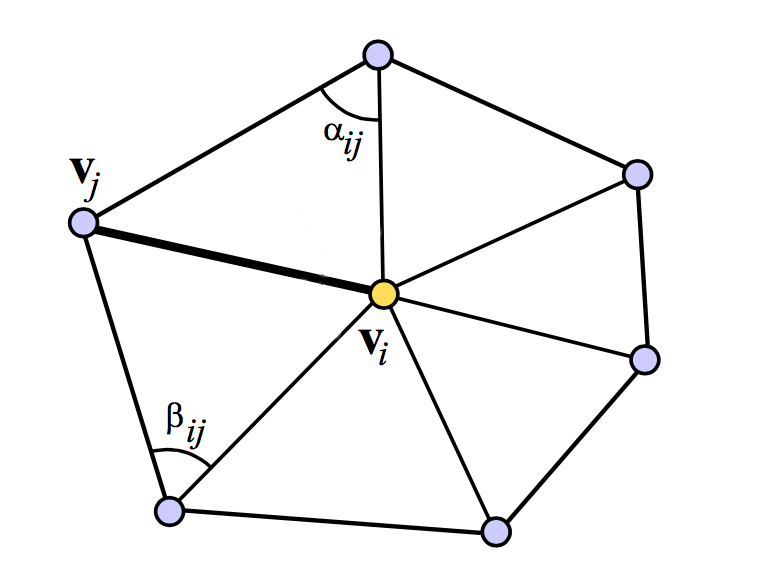
\includegraphics[width=0.5\textwidth]{cot.png}
        \caption{Cotangent formula (figure adopted from \cite{sorkine2005laplacian})}\label{fig:cot}
\end{figure}

Let $f: V \rightarrow \mathbb{R}$ be a discrete function on the triangle mesh. The Laplacian $\Delta_S f$ of $f$ at $V_i$ is:
$$
(\Delta_S f)(V_i) = \sum_{V_j \in N(V_i)} ( \cot \alpha_{ij} + \cot_{ij} ) (f(V_j) - f(V_i)).
$$
It is called ``cotangent formula''\cite{pinkall1993computing} for the discrete Laplace-Beltrami operator.

The discrete Laplace-Beltrami operator of the triangle mesh can be written as an $n$-by-$n$ symmetric matrix $L$ defined as
\begin{align*}
L_{ij} & = 
\begin{cases}
0 & \text{ if } V_i \text{ is not connected to } V_j \\
\cot \alpha_{ij} + \cot \beta_{ij} & \text{ if } V_i \text{ is connected to } V_j
\end{cases} \\
L_{ii} & = - \sum_{j \neq i} L_{ij}
\end{align*}

Let $(u_i, v_i)' = f(V_i)$. Let $\mathbf{u} = (u_1, \dots, u_n)'$ and $\mathbf{v} = (v_1, \dots, v_n)'$. The Laplace equation $(\Delta_S f)(V_i) = 0$ for all $V_i \in V$ can be written as
\begin{align*}
\begin{cases}
L\mathbf{u} = \mathbf{0} \\
L\mathbf{v} = \mathbf{0}.
\end{cases}
\end{align*}
Let $\mathbf{x} =  (u_1, \dots, u_n, v_1, \dots, v_n )$. Then we need to solve
\[
Q \mathbf{x} = \mathbf{0} \quad \text{ where }
Q =
\begin{pmatrix}
L & O_n \\
O_n & L
\end{pmatrix}
\text{ is a symmetric matrix.}
\]



\subsection{Boundary condition}

The boundary condition $f(\partial S) = \partial \mathbb{D}$ can be written as $u_k^2 + v_k^2 = 1$ for all $V_k \in V \cap \partial S$. Note that those are quadratic constraints on $\mathbf{x}$. There exists $2n$-by-$2n$ symmetric matrices $H_k$ such that $\mathbf{x}' H_k \mathbf{x} = u_k^2 + v_k^2$. Let $n_b$ be the number of boundary vertices $V \cap \partial S$. We have $n_b$ many quadratic constraints:
$$
\mathbf{x}' H_k \mathbf{x} = 1 \quad \text{ for } k = 1, \dots, n_b.
$$

Beside the boundary condition on the unit circle, we also need some another constraint for practical reason. It is intuitive that the solution of conformal parameterization is not unique, as any rigid motion on the mesh preserves all angle. Also, the constant mapping, i.e. $u_1 = u_2 = \dots = u_n$ and $v_1 = v_2 = \dots = v_n$, is a trivial solution. Therefore, in order to get rid of the above situation, we will need to fix at least three vertices to three different coordinates. Suppose we want to fix $(u_{l_1}, v_{l_1}) = (b_1, b_2)$, $(u_{l_2}, v_{l_2}) = (b_3, b_4)$ and $(u_{l_3}, v_{l_3}) = (b_5, b_6)$, where $(b_1, b_2) , (b_3, b_4) \text{ and } (b_5, b_6) \in \mathbb{D}$ are fixed coordinates. We have the following linear constraint:
$$
A\mathbf{x} = \mathbf{b} \quad \text{ where } A \text{ is such that } A\mathbf{x} = (u_{l_1}, v_{l_1}, u_{l_2}, v_{l_2}, u_{l_3}, v_{l_3} )' \text{ and } \mathbf{b} = (b_1, b_2, b_3, b_4, b_5, b_6)'
$$

In summary, we have $2n$ many quadratic constraints and also $4$ linear constraints.

\section{Optimization problem}

The conformal parameterization can be written as a triangle mesh with a parameterization function $f: S \rightarrow \mathbb{R}^2$
\begin{align*}
V & = \{ V_i \in S\}_{i = 1}^{n} & \text{Vertex}\\
T & = \{ (V_{t_1}, V_{t_2}, V_{t_3}) \} & \text{Triangulation}\\
f(V) & = \{ (u_i, v_i) \in \mathbb{R}^2 \}_{i = 1}^{n} & \text{Coordinates of vertices in }\mathbf{R}^2
\end{align*}

Given a triangle mesh $(V, T)$ of a surface $S$, we want to find the parameterization function $f(V) = \{ (u_i, v_i) \in \mathbb{R}^2 \}_{i = 1}^{n}$. Let $\mathbf{x} = (u_1, \dots, u_n, v_1, \dots, v_n)$. $\mathbf{x}$ is the solution of the following optimization problem:
\begin{equation}
\min_{\mathbf{x} \in \mathbb{R}^{2n} } \mathbf{x}'Q \mathbf{x} \qquad \text{subject to }
\begin{cases}
\mathbf{x}'H_k \mathbf{x} = 1 & \text{ for } k = 1, \dots, n_b \\
A \mathbf{x} = \mathbf{b} &
\end{cases} \tag{$\star$}
\end{equation}
where $Q$, $H_k$, $A$ and $\mathbf{b}$ are defined in the Section 3 \textbf{Discretization}. The optimization problem ($\star$) has a quadratic objective with quadratic constraints and linear constraints.

We apply augmented Lagrangian method to solve ($\star$).

The objective function, its gradient and its Hessian are:
\begin{align*}
\text{Obj}(\mathbf{x}) & = \mathbf{x}'Q \mathbf{x}  \\
\text{Grad}(\mathbf{x}) & = Q\mathbf{x}  \\ 
\text{Hess}(\mathbf{x}) & = Q
\end{align*}
The constraint function $c(\mathbf{x})$, gradient of constraint $\nabla c(\mathbf{x})$ and Hessian of constraint $\{ \nabla^2 c_k(\mathbf{x}) \}$ are:
\begin{align*}
c(\mathbf{x}) & = 
\begin{bmatrix}
\frac12 \mathbf{x}'H_1 \mathbf{x} \\
\vdots \\
\frac12 \mathbf{x}'H_{n_b} \mathbf{x} \\
A\mathbf{x} - \mathbf{b}
\end{bmatrix}
\\
\nabla c(\mathbf{x}) & = 
\begin{bmatrix}
H_1 \mathbf{x} & \dots & H_{n_b} \mathbf{x} & A'
\end{bmatrix}
\\
\{ \nabla^2 c_k(\mathbf{x}) \} & = 
\{ H_1, \dots, H_{n_b}, O_n, \dots, O_n \}
\end{align*}

The augmented Lagrangian, its gradient and its Hessian are:
\begin{align*}
L_\rho ( \mathbf{x}, \mathbf{y}) & =  
\mathbf{x}' Q \mathbf{x} - \mathbf{y}' c(\mathbf{x}) + \frac{\rho}{2} c(\mathbf{x})' c(\mathbf{x}) \\
\nabla_x L_\rho ( \mathbf{x}, \mathbf{y}) & = 
Q \mathbf{x} - [\nabla c(\mathbf{x})] \mathbf{y} + \rho [\nabla c(\mathbf{x})] c(\mathbf{x}) \\
\nabla^2_{xx} L_\rho ( \mathbf{x}, \mathbf{y}) & = 
Q - \sum_{k = 1}^{n_b + 6} \nabla^2 c_k(\mathbf{x}) \cdot y_k + \rho \sum_{k = 1}^{n_b + 6} \cdot c_k (\mathbf{x}) + \rho [\nabla c(\mathbf{x})] [\nabla c(\mathbf{x})]'
\end{align*}

With the above explicit formulas, we apply the augmented Lagrangian method with Newton's method to solve $(\star)$. See \text{Algorithm 1}.

\begin{algorithm}[H]
 $k = 0$, $\mathbf{x}_0 = \mathbf{0}$, $\mathbf{y}_0 = \mathbf{0}$, $\rho_k = 10$ \;
 \While{$\| c(\mathbf{x}_k) \| > \epsilon$ or $\| \text{Grad}(\mathbf{x}_k) - [\nabla c (\mathbf{x}_k)] \mathbf{y}_k \| > \epsilon$}{
  $\mathbf{x}_{k+1} = \min_{x} L_{\rho^k}(\mathbf{x} , \mathbf{y}_k)$ (by Newton's method) \;
  $k = k + 1$ \;
  \eIf{ $\| c(\mathbf{x}_k) \| \leq 0.000001 / 2^k$ }{
   $\rho_k = \rho_{k-1}$\;
   $\mathbf{y}_k = \mathbf{y}_{k-1} - \rho c(\mathbf{x}_k)$ \;
   }{
    $\rho_k = 2 \rho_{k-1}$ \;
    $\mathbf{y}_k = \mathbf{y}_{k-1}$ \;
  }
 }
 \caption{Augmented Lagrangian method}
\end{algorithm}

\section{Numerical experiment}

The implementation is done in Julia. See Section 8 \textbf{Appendix} for the codes.

Below is the numerical experiment of the surface mesh shown in Figure 1. The surface mesh consists of 88 vertices, in which 31 vertices are at boundary. The augmented Lagrangian method takes 11 iterations to converge.

\begin{center}
\begin{tabular}{ |r|r|r|r| } 
 \hline
 Iteration & $\rho$ & $\| c(\mathbf{x}_k) \|$ & $\| \text{Grad}(\mathbf{x}_k) - [\nabla c (\mathbf{x}_k)] \mathbf{y}_k \|$ \\
 \hline
     1 &    10 &    0.219869662769 &    3.474162683887 \\
     2 &    20 &    0.110261610250 &    2.182805069440 \\
     3 &    40 &    0.055224136741 &    2.225978483471 \\
     4 &    80 &    0.027637315846 &    2.247778475219 \\
     5 &   160 &    0.013825249327 &    2.258770957372 \\
     6 &   320 &    0.006914310456 &    2.264297284670 \\
     7 &   640 &    0.003457581625 &    2.267069021520 \\
     8 &  1280 &    0.001728898043 &    2.268457178338 \\
     9 &  2560 &    0.000864475909 &    2.269151847922 \\
    10 &  2560 &    0.000000148032 &    0.000000000001 \\
    11 &  2560 &    0.000000000201 &    0.000000000002 \\
 \hline
\end{tabular}
\end{center}

\section{Further work}

In this project, we only consider the surface mesh which is topologically equivalent to unit disk. We may work on surface with different topological type. Spherical parameterization is another problem we can investigate. Given a surface which is topologically equivalent to sphere, we want to find a parameterization on the unit sphere. It is also sensible to talk about conformal parameterization in this case. In further work, the method in this project will extended for conformal parameterization on unit sphere.


\bibliographystyle{plain}
\bibliography{report}

\section{Appendix}

The Julia notebook of the codes is on \url{https://github.com/pochoi/mat258A}.

\subsection{Functions to construct objective and constraints}
\begin{lstlisting}
function getBoundary(t)
    nt = size(t)[2]
    edge_list = Array{Int64,1}[]
    for i in 1:nt
        push!(edge_list, t[1:2,i])
        push!(edge_list, t[2:3,i])
        push!(edge_list, t[[3,1],i])
    end
    boundary_list = Array{Int64,1}[]
    for i in 1:length(edge_list)
       myedge = edge_list[i][[2,1]]
        if !in(myedge, edge_list)
            push!(boundary_list, edge_list[i])
        end
    end 
    boundary = zeros(Int64, length(boundary_list))
    boundary[1] = boundary_list[1][1]
    for i in 1:length(boundary)
       if i == length(boundary_list) 
           break
       end
        for j in 1:length(boundary_list)
            if boundary_list[j][1] == boundary[i]
             boundary[i+1]  = boundary_list[j][2]
             break
            end
        end
    end
    return boundary
end

function getEdge(p, t)
    e1 = p[:, vec(t[3,:])] - p[:, vec(t[2,:])]
    e2 = p[:, vec(t[1,:])] - p[:, vec(t[3,:])]
    e3 = p[:, vec(t[2,:])] - p[:, vec(t[1,:])]
    e1norm = vec(sqrt(sum(e1.^2, 1)))
    e2norm = vec(sqrt(sum(e2.^2, 1)))
    e3norm = vec(sqrt(sum(e3.^2, 1)))
    return e1, e2, e3, e1norm, e2norm, e3norm
end

function mesh_cot(p, t)
    (e1, e2, e3, e1norm, e2norm, e3norm) = getEdge(p, t)
   e1cos = vec(sum(-e2 .* e3, 1)) ./ e2norm ./ e3norm
   e2cos = vec(sum(-e3 .* e1, 1)) ./ e3norm ./ e1norm
   e3cos = vec(sum(-e1 .* e2, 1)) ./ e1norm ./ e2norm
    r1 = zeros(Float64, size(t)) 
    r2 = zeros(Float64, size(t)) 
    r3 = zeros(Float64, size(t)) 
    for i in 1:size(t)[2]
      r1[:,i] = cross(e2[:,i], e3[:,i])  
      r2[:,i] = cross(e3[:,i], e1[:,i])  
      r3[:,i] = cross(e1[:,i], e2[:,i])  
    end
   e1sin = vec(sqrt(sum(r1.^2,1))) ./ e2norm ./ e3norm
   e2sin = vec(sqrt(sum(r2.^2,1))) ./ e3norm ./ e1norm
   e3sin = vec(sqrt(sum(r3.^2,1))) ./ e1norm ./ e2norm
   e1cot = e1cos ./ e1sin;
   e2cot = e2cos ./ e2sin;
   e3cot = e3cos ./ e3sin;
   return vec(e1cot), vec(e2cot), vec(e3cot)
end

function WCot(p, t)
    n = size(p)[2]
    (e1cot, e2cot, e3cot) = mesh_cot(p, t);
    I = [vec(t[2,:]); vec(t[3,:]); vec(t[1,:])]
    J = [vec(t[3,:]); vec(t[1,:]); vec(t[2,:])]
    S = [e1cot; e2cot; e3cot]
    W = sparse(I,J,S, n, n)
    #Wfull = Float64[ W[i,j] for i in 1:n, j in 1:n]
    return W
end

function LCot(p, t)
    n = size(p)[2]
    W = WCot(p,t)
    W = W + transpose(W)
    L = sparse(1:n, 1:n, vec(sum(W,2))) - W
    #Lfull = Float64[ L[i,j] for i in 1:n, j in 1:n]
    return L
end

function areaMixMeyer(p, t)
    n = size(p)[2]
    (e1, e2, e3, e1norm, e2norm, e3norm) = getEdge(p, t)
    (e1cot, e2cot, e3cot) = mesh_cot(p, t);
    I = [vec(t[2,:]); vec(t[3,:]); vec(t[1,:])]
    J = [vec(t[3,:]); vec(t[1,:]); vec(t[2,:])]
    S = [e1cot .* vec(e1norm).^2; e2cot .* vec(e2norm).^2; e3cot .* vec(e3norm).^2]
    tri_angle = meshAngle(v,f)
    obtuse_flag = vec(any(tri_angle .> pi/2 , 1))
    #obtuse_flag = (e1angle > pi/2) | (e2angle > pi/2) | (e3angle > pi/2)
    tri_area, v_area = meshArea(p, t)
    tri_ring = vertexTriRing(p, t)
    mix_area = zeros(Float64, n) 
    for i in 1:n
        a = 0
        for itri in tri_ring[i]
            v_index = find(t[:,itri] .== i)[]
            if !obtuse_flag[itri]
                a += v_area[v_index, itri]
            else
                a += tri_area[itri] / ( (tri_angle[v_index,itri] > pi/2) ? 2 : 4)
            end
        end
        mix_area[i] = a
    end
    return mix_area
end

immutable ConfOpt
    Q::SparseMatrixCSC{Float64,Int64}
    H::Array{SparseMatrixCSC{Float64,Int64},1}
    A::Array{SparseMatrixCSC{Float64,Int64},1}
    b::Array{Float64,1}
    n::Int64
    m::Int64
    objFun::Function
    objGrad::Function
    objHess::Function
    constrFun::Function
    constrGrad::Function
    constrHess::Array{Function,1}
    augLagFun::Function
    augLagGrad::Function
    augLagHess::Function
    x0::Array{Float64,1}
    p::Array{Float64,2}
    t::Array{Int64,2}
    boundary::Array{Int64,1}
    boundary_3point::Array{Int64,1}
    boundary_3point_v::Array{Float64,2}
end

function Ltut(p, t)
	n = size(p)[2]
    I = [vec(t[2,:]); vec(t[3,:]); vec(t[1,:])]
    J = [vec(t[3,:]); vec(t[1,:]); vec(t[2,:])]
    S = ones(length(I))
    W = sparse(I,J,S, n, n)
    W = W + transpose(W)
    L = sparse(1:n, 1:n, vec(sum(W,2))) - W
    
    boundary = getBoundary(t)
    nb = length(boundary)
    theta = (2pi/nb) * (0:(nb-1))

	b1 = zeros(Float64, n)
	b2 = zeros(Float64, n)

	for k = 1:nb
		b1 = b1 - L[:, boundary[k]] * cos(theta[k])
		b2 = b2 - L[:, boundary[k]] * sin(theta[k])
	end
	b1[boundary] = cos(theta)
	b2[boundary] = sin(theta)

	Lw = copy(L)
	Lw[:, boundary] = 0
	Lw[boundary,:] = 0
	for k = 1:nb
		Lw[boundary[k],boundary[k]] = 1
	end

	uv = Lw \ [b1 b2]
	return uv
end


function ConfOpt(p::Array{Float64,2}, t::Array{Int64,2})
    n = size(p,2)
    boundary = getBoundary(t)
    nb = length(boundary)

    Qraw = LCot(p,t)
    Q = [Qraw zeros(n,n); zeros(n,n) Qraw]

	H = Array{Float64,2}[]
	for i in 1:nb
		G = zeros(Float64, 2, 2n)
		G[1,boundary[i]] = 1
		G[2,n + boundary[i]] = 1
		Hi = G.' * G
		push!(H, Hi)
	end

    objFun = function(x::Array{Float64,1}) 0.5 * getindex(x.' * Q * x, 1) end
    objGrad = function(x::Array{Float64,1}) Q * x end
    objHess = function(x::Array{Float64,1}) Q end

    theta = (2pi/3) * [0;1;2]
    boundary_3point = boundary[[1, 1 + div(nb,3), 1 + div(nb,3)*2]]
    boundary_3point_v = [cos(theta).'; sin(theta).']

    A = [zeros(Float64, 1, 2n) for i in 1:6]
    b = zeros(Float64, 6)
    for i in 1:3
    	A[i][1, boundary_3point[i]] = 1
    	A[3+i][1, boundary_3point[i] + n ] = 1
    	b[i] = cos(theta[i])
    	b[3+i] = sin(theta[i])
    end

    constrFun = function(x::Array{Float64,1}) 
    	[Float64[ 0.5* ((x.' * H[i] * x) - 1)[] for i in 1:nb];
    	Float64[ ((A[i] * x) - b[i])[] for i in 1:6]]
	end
    constrGrad = function(x::Array{Float64,1})
    	J = zeros(Float64, 2n, nb+6)
    	for i in 1:nb
	    	J[:,i] = H[i] * x
	    end
	    for i in 1:6
	    	J[:, nb + i] = A[i].'
	    end
    	return J
	end
    constrHess = Function[]
    for i in 1:nb
    	fun = function(x::Array{Float64,1}) H[i] end
    	push!(constrHess, fun)
    end
    for i in 1:6
    	fun = function(x::Array{Float64,1}) zeros(Float64,2n,2n) end
    	push!(constrHess, fun)
    end

    augLagFun = function(x::Array{Float64,1}, y::Array{Float64,1}, rho::Float64)
    	objFun(x) - dot(y, constrFun(x)) + 0.5rho * dot(constrFun(x),constrFun(x))
	end
	augLagGrad = function(x::Array{Float64,1}, y::Array{Float64,1}, rho::Float64)
    	objGrad(x) - constrGrad(x) * y + rho * constrGrad(x) * constrFun(x)
	end
	augLagHess = function(x::Array{Float64,1}, y::Array{Float64,1}, rho::Float64)
		Q - sum(H .* y[1:nb]) + rho * sum(H .* constrFun(x)[1:nb]) + rho * constrGrad(x) * transpose(constrGrad(x))
	end

	uv = Ltut(p, t)
	x0 = [uv[:,1];uv[:,2]]

    return ConfOpt(Q, H, A, b, 2n, nb+6,
    			objFun, objGrad, objHess,
    			constrFun, constrGrad, constrHess,
    			augLagFun, augLagGrad, augLagHess,
    			x0, p, t, boundary, boundary_3point, boundary_3point_v)
end


function augLagObj(prob::ConfOpt, y::Array{Float64,1}, rho::Float64)
	augLagFun = function(x::Array{Float64,1})
    	prob.objFun(x) - dot(y, prob.constrFun(x)) + 0.5rho * dot(prob.constrFun(x), prob.constrFun(x))
	end
	augLagGrad = function(x::Array{Float64,1})
    	prob.objGrad(x) - prob.constrGrad(x) * y + rho * prob.constrGrad(x) * prob.constrFun(x)
	end
	augLagHess = function(x::Array{Float64,1})
		prob.Q - sum(prob.H .* y[1:(prob.m-6)]) + rho * sum(prob.H .* prob.constrFun(x)[1:(prob.m-6)]) + rho * prob.constrGrad(x) * transpose(prob.constrGrad(x))
	end

	obj = function(x::Array{Float64,1}) 
		return augLagFun(x), augLagGrad(x), augLagHess(x)
	end

	return obj
end

\end{lstlisting}

\subsection{Newton's methods and augmented Lagrangian method}
\begin{lstlisting}
# Newton Method
function newtmin(obj, x0; maxIts=1000, optTol=1e-6, BkFlag = false, btFlag = true)
    # Minimize a function f using Newton’s method.
    # obj: a function that evaluates the objective value,
    # gradient, and Hessian at a point x, i.e.,
    # (f, g, H) = obj(x)
    # x0: starting point.
    # maxIts (optional): maximum number of iterations.
    # optTol (optional): optimality tolerance based on
    # ||grad(x)|| <= optTol*||grad(x0)||
    # BkFlag (optional): true for doing Modified Hessian
    # btFlag (optional): true for doing Back Tracking
    f0, g0, H0 = obj(x0)
    its = 0
    Opt = Float64[]
    xkp = copy(x0)
    for i in 1:maxIts
        xk = copy(xkp)
        fk, gk, Hk = obj(xk)
        opt = norm(gk, 2)
        push!(Opt, opt)
        #if opt < optTol*norm(g0)
        if opt < optTol
            break
        end
        if BkFlag == true
            Bkinv = BkFunInv(Hk, 0.01)
            dk = Bkinv * (- gk)
        else
            dk = Hk \ (- gk)
        end
        if btFlag == true
            αk = backTracking(obj, xk, dk, gk)
        else
            αk = 1
        end
        xkp = xk + αk * dk
        its = its + 1
    end
    return xkp, its, Opt
end

function AugLag(prob::ConfOpt; maxItr=20, optTolck = 1e-8, optTolKKT = 1e-8, rho0 = 10.0)
	y0 = zeros(Float64, prob.m)
	
	rhok = rho0
	yk = copy(y0)
	xk = copy(prob.x0)
    #xk = zeros(Float64, prob.n)

    rho_counter = 0
	counter = 0    
    
    @printf "%6s %6s %18s %18s" "Itr" "rho" "Norm Constr" "Norm AugLag Grad\n"
    storage_cnorm = Float64[]
    storage_lnorm = Float64[]
	for itr = 1:maxItr
		
		xkp = newtmin(augLagObj(prob, yk, rhok), xk, maxIts=20, optTol = (1e-4 / 10^itr ) )[1]
        push!(storage_cnorm, norm(prob.constrFun(xkp)))
        push!(storage_lnorm, norm(prob.objGrad(xk) - prob.constrGrad(xk) * yk))
        @printf "%6d %6.0f %18.12f %18.12f\n" itr rhok storage_cnorm[end] storage_lnorm[end] 
            if norm(prob.constrFun(xkp)) < 1e-3 * (1/2)^rho_counter
			rhokp = rhok
			ykp = yk - rhokp * prob.constrFun(xkp)
			rho_counter = rho_counter + 1
		else
			rhokp = 2.0 * rhok
			ykp = copy(yk)
		end

		rhok = rhokp
		yk = copy(ykp)
		xk = copy(xkp)

		counter = itr
		if (norm(prob.constrFun(xkp)) < optTolck) & (norm( prob.objGrad(xk) - prob.constrGrad(xk) * yk) < optTolKKT)
			break
		end
	end

    return xk, yk, rhok, counter, storage_cnorm, storage_lnorm
end
\end{lstlisting}

\subsection{How to run the codes}
\begin{lstlisting}
f = readdlm("test1_f.dat", ',', Int64)
v = readdlm("test1_v.dat", ',', Float64)

f = f.';
v = v.';

myprob = ConfOpt(v, f);
result_x = AugLag(myprob, maxItr=50);
\end{lstlisting}

\end{document}
